\chapter{大规模机器学习框架}\label{chap:large-scale-distributed-deep-learning}
\addtocontents{los}{\protect\addvspace{10pt}}

\begin{intro}
本章内容主要是对知乎上\textit{carbon zhang}的专栏文章\textbf{大规模机器学习框架的四种境界}%
\footnote{https://zhuanlan.zhihu.com/p/29968773}%
进行的总结与整理。
\end{intro}

\section{背景}\label{sec:background}

自从 Google 发表著名的 GFS%
\footnote{The Google File System}、%
MapReduce%
\footnote{MapReduce: Simplified Data Processing on Large Clusters}、%
Big Table% 
\footnote{Bigtable: A Distributed Storage System for Structured Data}%
三篇 paper 以后,互联网正式迎来了大数据时代。

有了 GFS,即分布式文件系统,我们有能力积累海量的数据样本,比如在线广告的曝光和点击数据,天然具有正负样本的特性,
积累一两个月往往就能轻松获得百亿、千亿级的训练样本。这样海量的样本如何存储?用什么样的模型可以学习海量样本中有用
的模式(patterns)?这些问题不止是工程问题,也值得每个做算法的同学去深入思考。

\begin{newnote}[GFS]
Google 在 2003 年发表 GFS 论文,对其中的 Falut Tolerance 有很深刻的印象(第一遍看 GFS 论文的时候)。
\end{newnote}

\begin{newnote}[BigTable]
BigTable 是什么?那篇论文我还没有看过。
\end{newnote}

\subsection{简单模型 or 复杂模型}\label{subsec:simple-or-complex}

在深度学习概念提出之前,我们大都使用的是传统的机器学习算法,例如 LR(逻辑回归)、SVM(支持向量机)、感知机等,这些算法种类很少且相对固定;
那时候要解决一个实际的问题,更多的工作主要集中在\textbf{特征工程}方面。而特征工程本身并没有很系统化的指导理论
(至少目前没有看到系统介绍特征工程的书籍),所以很多时候特征的构造技法显得光怪陆离,是否有用也取决于问题本身、数据样本、模型以及\textbf{运气}。

如果给这种方式起一个名字的话,大概是简单模型+复杂特征;简单模型说的是算法比如 LR、SVM 本身并不复杂,参数和表达能力基本呈现一种线性关系,
易于理解;复杂特征则是指特征工程方面不断尝试使用各种奇技淫巧构造的可能有用、可能没用的特征。这部分特征的构造方式可能会有各种 trick,
比如窗口滑动、离散化、归一化、开方、平方、笛卡尔积、多重笛卡尔积等等;因为特征工程本身并没有特别系统的理论和总结,因此需要大量阅读和自己
业务场景一样或类似的 paper,从里面学习作者分析、理解数据的方法以及对应的构造特征的技法,久而久之,有望形成自己的知识体系。

深度学习概念提出以后,人们发现通过深度神经网络可以进行一定程度的表示学习(representation learning),例如在图像领域,通过 CNN 提取
图像特征(feature) 并在此基础上进行分类,此方法(AlexNet%
\footnote{ImageNet Classification with Deep Convolutional Neural Networks}%
)一举打破了之前算法的天花板,而且是以极大的差距打破。这给所有算法工程师带来了新的思路,既然深度学习本身有提取特征的能力,
干嘛还要苦苦的自己去做人工特征设计呢?

\begin{newnote}[AlexNet]
AlexNet
\end{newnote}

深度学习虽然一定程度上缓解了特征工程的压力,但这里要强调两点:
\begin{enumerate}
\item 缓解并不等于彻底解决。除了图像这种特定领域,在个性化推荐等领域,深度学习目前还没有完全取得绝对的优势;究其原因,可能还是数据自身
内在结构的问题,使得在其他领域目前还没有发现类似图像 + CNN 这样的完美 CP。
\item 深度学习在缓解特征工程的同时,也带来了模型复杂、不可解释的问题。算法工程师在网络结构设计方面一样要花很多心思来提升效果。
\end{enumerate}
概括起来,深度学习代表的简单特征+复杂模型是解决实际问题的另一种方式。

两种模式孰优孰劣还难有定论,以点击率预测为例,在计算广告领域往往以海量特征 + LR 为主流,根据 VC 维理论,LR 的表达能力和特征个数成正比,因此
海量的 feature 也完全可以使 LR 拥有足够的描述能力。而在个性化推荐领域,深度学习刚刚萌芽,目前 google play 采用了 WDL 的结构
\footnote{Wide~\& Deep Learning for Recommender Systems},
YouTube 采用了双重 DNN 的结构\footnote{Deep Neural Networks for YouTube Recommendations}。

\begin{newnote}[VC 维理论]
待补充
\end{newnote}

不管是哪种模式,当模型足够庞大的时候,都会出现模型参数一台机器无法存放的情况。比如百亿级 feature 的 LR 对应的权重 $w$ 有好几十个 G,
这在很多单机上存储都是困难的,大规模神经网络则更复杂,不仅难以单机存储,而且参数和参数之间还有逻辑上的强依赖,要对超大规模的模型进行训练势必
要借用分布式系统的技法,本文主要是系统总结这方面的一些思路。

\begin{newnote}[VGG16 每一层参数所占的空间大小]
待补充 https://zhuanlan.zhihu.com/p/31558973
\end{newnote}

\subsection{数据并行 vs 模型并行}\label{subsec:data-vs-model}

数据并行和模型并行是理解大规模机器学习框架的基础概念,这两个概念在知乎问题『谈谈你对“GPU/CPU 集群下做 Data/Model Parallelism 的区别”的理解?%
\footnote{https://www.zhihu.com/question/31999064}%
』中沐帅给出了一个非常直观且经典的解释:
\begin{quotation}
举个栗子。假设我准备盖一座双子楼,我有两个选择:一个是把人分成两组,每组建一栋楼然后装修好,最后把两个连起来。二是仍然分两组,
第一组先把楼盖好,第二组负责装修。

第一个方案的好处是并行度高。但要求每个组又要懂建房又要懂装修。第二方案要求低点,一个组会建,一个组会装修就行了。坏处是,一个组在干活的时候
另外一个组可能在赋闲。

换成“data/model parallelism”, 这里一个组是一个 cpu 或者一个 gpu。第一个方案是 data parallelism,第二方案是 model parallelism。
技能要求可以简单看成是对内存的需求。当模型很大不能 fit 进单机内存或者单 GPU 内存(这个可能性高多了)的时候,我们一般用 model parallelism,
不然用 data parallelism,因为通常快一些。但某些情况下,model parallelism 的并行程度也没那么低,例如 deep neural network。
换回到那个栗子,每一层楼就是 neural network 的一层。这时候我可以流水盖楼:

第一天:一组盖第一层

第二天:一组盖第二层,二组装修第一层

第三天:一组盖第三层,二组装修第二层$\cdots$

或者只要楼高,可以基本接近2倍加速。
\end{quotation}
第一个方案和数据并行类似,第二个方案则道出了模型并行的精髓。

数据并行理解起来比较简单,当样本比较多的时候,为了使用所有样本来训练模型,不妨把数据分布到不同的机器上,然后每台机器都来对模型参数进行迭代,如图
\ref{fig:data-parallelism} 所示:

\begin{figure}[!hbtp]
\centering
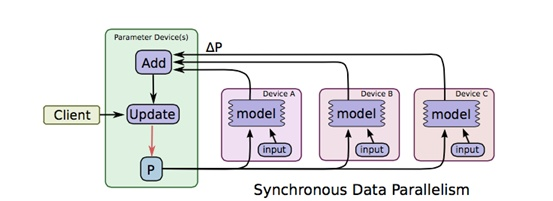
\includegraphics[width=0.85\textwidth]{data-parallelism}
\caption{数据并行}
\label{fig:data-parallelism}
\end{figure}

图片取材于 TensorFlow 的 paper%
\footnote{TensorFlow:Large-Scale Machine Learning on Heterogeneous Distributed Systems},
图中 ABC 代表三台不同的机器,上面存储着不同的样本,模型 P 在各台机器上计算对应的增量 $\Delta$P,然后在参数存储的机器上进行汇总和更新,这就是数据并行。先忽略 synchronous,这是同步机制相关的概念,在第 \ref{subsec:ps-synchronous} 节会有专门介绍。

数据并行概念简单,而且不依赖于具体的模型,因此数据并行机制可以作为框架的一种基础功能,对所有算法都生效。与之不同的是,模型并行因为参数间存在依赖关系
(其实数据并行中参数更新也可能会依赖所有的参数,但区别在于往往是依赖于上一个迭代的全量参数。而模型并行往往是同一个迭代内的参数之间有强依赖关系,比如
DNN 网络的不同层之间的参数依照 BP 算法形成的先后依赖),无法类比数据并行这样直接将模型参数分片而破坏其依赖关系,所以模型并行不仅要对模型分片,
同时需要调度器来控制参数间的依赖关系。而每个模型的依赖关系往往不同,所以模型并行的调度器因模型而异,较难做到完全通用。关于这个问题,CMU 的 Erix Xing 在这里%
\footnote{https://www.jianshu.com/p/00736aa21dc8}
有所介绍,感兴趣的可以参考。

\begin{newnote}[CMU Erix Xing 的分享]
待补充,有文字版整理以及演讲的 PPT
\end{newnote}

\begin{newnote}[现在模型并行的必要性]
ResNet50 模型的整个参数是 100M 左右?现在没有模型并行的需求?全连接层的去除?大家都是在使用着数据并行?

必要性?
\end{newnote}

\begin{newnote}[对于模型并行的调研或相关论文可以推后]
先考察一下现在模型并行的必要性,再开始接触这方面的论文。
\end{newnote}

\noindent\rule[0.25\baselineskip]{\textwidth}{1pt}

模型并行的问题定义可以参考 Jeff Dean 这篇 paper
\footnote{Large Scale Distributed Deep Networks}
,其作为 TensorFlow 的前身,其中图:

\begin{figure}[hbtp]
\centering
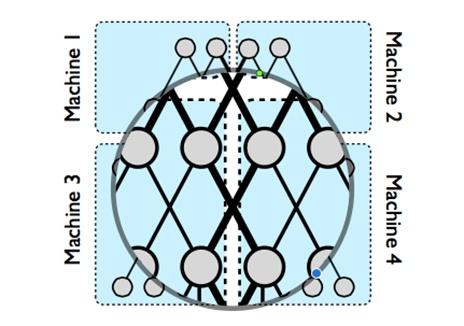
\includegraphics[width=0.6\textwidth]{model-parallelism}
\caption{模型并行}
\label{fig:model-parallelism}
\end{figure}

解释了模型并行的物理图景,当一个超大神经网络无法存储在一台机器上时,我们可以切割网络存到不同的机器上,但是为了保持不同参数分片之间的依赖,
如图中粗黑线的部分,则需要在不同的机器之间进行 concurrent 控制;同一个机器内部的参数依赖,即图中细黑线部分在机器内即可完成控制。

黑线部分如何有效控制呢?如下图所示:

\begin{figure}[hbtp]
\centering
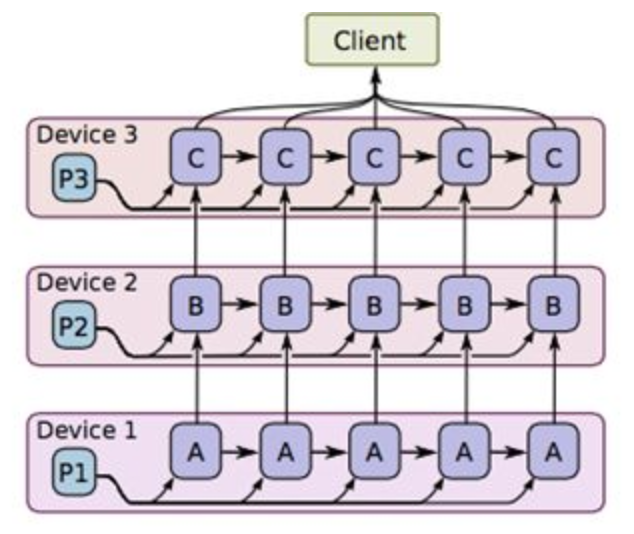
\includegraphics[width=0.6\textwidth]{model-parallelism-training}
\caption{模型并行中的训练过程}
\end{figure}

在将模型切分到不同机器以后,我们将参数和样本一起在不同机器间流转,图中 ABC 代表模型的不同部分的参数;假设 C 依赖 B,B 依赖 A,机器 1 上得到 A 的一个迭代后,
将 A 和必要的样本信息一起传到机器 2,机器 2 根据 A 和样本对 P2 更新得到,以此类推;当机器 2 计算 B 的时候,机器 1 可以展开 A 的第二个迭代的计算。
了解 CPU 流水线操作的同学一定感到熟悉,是的,模型并行是通过数据流水线来实现并行的。想想那个盖楼的第二种方案,就能理解模型并行的精髓了。

\begin{figure}[hbtp]
\centering
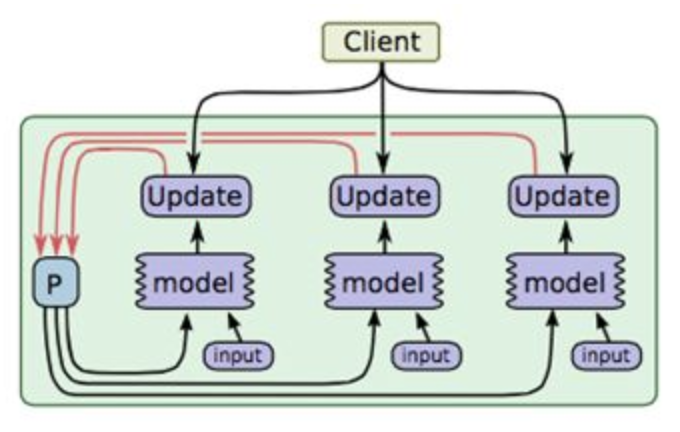
\includegraphics[width=0.65\textwidth]{concurrent-step}
\caption{Concurrent 控制}
\end{figure}

上图则是对控制模型参数依赖的调度器的一个示意图,实际框架中一般都会用 DAG(有向无环图)调度技术来实现类似功能,未深入研究,以后有机会再补充说明。

理解了数据并行和模型并行对后面参数服务器的理解至关重要,但现在让我先荡开一笔,简单介绍下并行计算框架的一些背景信息。

\noindent\textbf{待消化之后补充:}

GPU 上的数据/模型并行与 CPU 集群上的并没有本质区别。从 Fundamental 的角度来说,都是要解决几个问题:
\begin{enumerate}
  \item 通过并行化来做性能加速
  \item 把不可行变为可行(单机内存无法 hold 的 huge model size)
\end{enumerate}

从手段上来说,抽象来看都是这几种:
\begin{enumerate}
  \item 将计算与通信开销overlap以后,提高计算资源的utilization rate[1]
  \item 结合具体的的算法业务场景,对网络的拓扑结构进行优化,在不明显损失精度的情况下,减少并行计算的同步过程所需要传输的数据量
  (典型的例子就是 CNN 里卷积层的 local connectivity,weight sharing,以及 pooling 的设计理念[7])
  \item 将算法与系统相结合,在不明显损失精度的情况下,改善计算资源的utilization rate
  (典型的例子就是Hogwild为代表的ASGD算法[2]以及Eric Xing的团队提出的SSP[3])
\end{enumerate}

具体到操作层面,因为CPU与GPU在计算特点上的差异,还是会引入一些区别: 
\begin{enumerate}
  \item 相较于 CPU 而言,GPU 更强大的『naive』浮点算术能力(这里提到『naive』是为了突出 GPU 硬件设计上忽略复杂的控制结构,
  而把更多的芯片资源用于 computation intensive 的计算逻辑并辅之以 high latency/high bandwidth[8] 的显存资源,来获取到
  浮点计算吞吐能力的显著提升 --- no free lunch 的又一个典型 use case)使得它跟通信的性能 gap 要更为突显,也就使得 GPU 集群上,
  因为计算与通信的 gap 导致的性能 degradation 会更显著。在 GPU 集群里,引入高速通信链路(InfiniBand)以及特定的硬件技术支持
  (GPU Direct  RDMA[11])也都是为了缓解计算与通信的 gap(对于 GPU 与 CPU 计算能力的差异,既不能低估,也不应该过分高估,
  参见 Intel 发在 ISCA10 上的这篇文章[5])。
  \item GPU 的访存特点也使得 GPU 计算平台上能 hold 的有效模型尺寸通常来说是远小于 CPU 平台上的(以比较主流的 Nvidia Tesla K40M[6]为例,
  显存 12GiB),这也使得 GPU 平台上在处理比较大的模型的时候,会比 CPU 平台更早地遇到模型尺寸的瓶颈,需要考虑model parallelism。
  而 GPU 异构计算的复杂性和非黑盒特性也使得 GPU 平台上做 model parallelism 需要考虑更多的 constraint( global memory/shared memory/register file
  这些不同存储单元的延迟及带宽差异),相应会要求更为精巧的设计。
\end{enumerate}

总的来说,我个人以为 GPU 和 CPU 集群上的分布式机器学习系统的搭建并不存在本质上的差异,但是存在操作层面的区别。这些区别的有效
handle 非常依赖于强工程能力,特别是良好的体系结构背景与机器学习 common sense 的有效结合。具体来说,结合硬件的具体指标,
有效平衡好计算与通信的耗时比例,以及 CGMA(Computation to Global Memory Access) ratio[14],对于保证 GPU 集群上的程序性能
是有着重要帮助的。即便是有了 CUDA-Aware MPI[10](OpenMPI 从 1.7.4[12] 开始就已经既支持 InfiniBand 也支持 GPU Direct了),
让编程界面变得跟开发常规 MPI 程序更像了,但是对底层硬件性能指标的精确把握才可能让我们真正用好这些编程 API 完成分布式机器学习系统的开发工作。

再从一个更大的picture来看,分布式机器学习系统,本质上跟常规的分布式系统并没有差异。虽然在Eric Xing的文章[9]里提到了pure-system或pure-algorithm的视角看待分布式学习系统的limitation。但实际上从工业界应用的角度来看mitigate这个limitation所需要的代价其实并不会非常之高(我个人以为Xing教授在Large Scale Learning方面关于异步更新场景下收敛性证明的一些理论性工作对于分布式机器学习系统的未来演进有着方向性的重要意义和价值,但是仅从工业应用的角度来看还并没有构成严格的必要前提条件,有则更佳,欠乏其实并不会影响实际的业务推进和应用)。所以我还是会更愿意把分布式机器学习系统看成分布式系统在特定业务场景下的一个use case。有扎实的分布式系统经验的人,加以专门的Machline Learning相关的培训,其实并不难成长为分布式机器学习系统的专家(五年前,能够用MPI实现并行LR算法,可能还算是相当不错的技术成绩。而现在,一个基础扎实的应届生,给他合适的mentorship,其实花两三个月的时间也就能够实现一个可用于支持线上生产训练任务的版本了)。

现在,因为技能本身的diversity,拥有分布式机器学习系统开发经验的工程师还是稀缺资源,但是我会有这样一种感觉,随着时间的推移,人才的流动,会有更多的人能够掌握相关的经验技能,这个技能的稀缺性也会渐渐地下降到一个稳定值。大规模机器学习系统的Cross-domain性质所带来的固有难度还是存在一个固有的门坎,但是在我看来,这些门坎更多是一些know-how性质的门坎,而不是fundamental的门坎,是可以通过建立有效的培养机制来解决掉的。举例来说,不理解L1和L2正则为什么一个对应于Laplace先验,另一个对应于高斯先验,并不会影响我们去实现相应的分布式L1/L2 LR算法;同样,对矩阵分解理论缺乏精细的理解和把控,也不会构成我们去实现一个SVDFeature或是Tensor Decomposition算法的本质障碍;没有办法把EM算法的原理推敲得很清楚,也不会影响我们去实现一个并行版的PLSA主题模型。从工程实现的角度去完成一个academia community设计出来的大规模机器学习算法和自已从头设计一个大规模机器学习算法所需要的背景知识还是不一样的。前者更适合工业界的同学来完成,后者则更适合academia的同学来担当。(注意,我上面说的都是大规模算法的实现,而不是大规模算法的应用,我个人的观点,真正要把这些算法有效地应用到业务场景里,难度反而更大,不是仅仅靠良好的engineering practice和machline learning common sense就可以做到的,而会需要更扎实的数理统计以及数据挖掘/机器学习的专业背景)

个人来说,我更期待学术界能够从更fundamental的层面为large scale learning提供支持。因为现在的large scale learning系统在工业界的应用,我觉得还更多是一种以embarrassingly parallel为代表的暴力式方法带来性能优化。data parallelism/model parallelism不外如是,ASGD也算是一个“暴力”性质的例子(异步SGD虽然看起来很美,但是从实际的implementation上来看,在不同数据集上保证良好的收敛性并不是件容易的事情,在带来计算资源的更有效utilization rate的同时,ASGD固有的随机性其实让达到相同收敛点所需耗费的时间更长,变数也更多。G家的Paper[4]虽然claim说在non-convex, non-sparse场景下,他们使用ASGD+Adagrad也能够获得不错的收敛效果,但是缺失了严格的理论证明总会让人猜测有一些论文中没有透露的tricks才使得他们保证了ASGD在不同数据集上的收敛能力)。这种”暴力美学“性质的优化工业界有足够的能力去handle,而工业界因其自身定位特别是业务压力,未必有能力和精力handle的则是一些通过算法设计改良将算法时间复杂度或空间复杂度大幅降下来的case,典型的例子就是Newton法之于Gradient Descent,LBFGS算法之于原生的BFGS算法。以及对算法改良的theory justification,比如Eric Xing的团队在bounded delay场景下异步更新收敛性证明方面做过的一些工作。

最后简单summarize一下:
\begin{enumerate}
  \item GPU与CPU集群上Model/Data Parallelism不存在本质上的区别,更多是存在工程细节上的区别。对这些工程细节的有效handle依赖于强体系结构背景和机器学习 common sense的有机结合。
  \item 大规模机器学习系统本质上可以视为分布式系统的一个特例。虽然现在从事大规模机器学习系统开发还算是稀缺能力,但是开发大规模机器学习系统所需的技能经验是可以通过有效的培养机制加以养成的。
  \item 为了担心误导,特地加入对2的补充。只是开发出可以用于支持线上常规业务(CTR Prediction/搜索推荐/文本潜层语义挖掘,以及比较成熟的Deep Learning应用场景—Speech and CV)的大规模机器学习系统的技能经验是不难培养的,但是真正顶尖的相关能力则是不太容易培养的(似乎任何行当都是如此)。在资讯发达,行业交流频繁的年代,只是写一个可以work并支持线上业务基本需求的大规模并行算法并不存在本质困难(就算是一些现在不知道应该怎么做的算法,随着时间推移也不难从别人那里听说个大概,自然也就可以完成相应的实现了),但是结合业务场景,进行算法定制,来帮助业务建立起技术壁垒,就需要在engineering practice, machline learning common sense之外,对domain knowledge(既指代技术知识,也包括业务知识)建立起更深刻的理解和把握了,这种能力是需要通过长时间的思考,沉淀,持续地追踪最新的学术进展,同时touch多个domain才可能建立起来的,非量产品。
\end{enumerate}

\begin{itemize}
  \item [Alex2014] One Weird Trick for Parallelizing CNN
  \item [Niu2011] Hogwild!: A lock-free approach to parallelizing stochastic gradient descent 
  \item [Qirong2013] More Effective Distributed ML via a Stale Synchronous Parallel Parameter Server
  \item [Jeff2012]Large scale distributed deep networks 
  \item [Victor2010]Debunking the 100X GPU vs. CPU Myth: An Evaluation of Throughput Computing on CPU and GPU
  \item [Nvidia官网]http://www.nvidia.com/content/PDF/kepler/nvidia-tesla-k40.pdf
  \item [Jarret2009]What is the Best Multi-Stage Architecture for Object Recognition? 
  \item [Patterson]Why Latency Lags Bandwidth, and What it Means to Computing 
  \item [Eric2014]http://www.cs.cmu.edu/~epxing/talks/IEEE2014-BigData-Tutorial.pdf
  \item [Nvidia官网]NVIDIA GPUDirect https://developer.nvidia.com/gpudirect
  \item [Nvidia官网]http://on-demand.gputechconf.com/gtc/2013/presentations/S3047-Intro-CUDA-Aware-MPI-NVIDIA-GPUDirect.pdf
  \item [OpenMPI GitHub]https://github.com/open-mpi/ompi/
  \item [David B.Kirk2013]Programming Massively Parallel Processors, 2nd Edition, Chapter 5, Section 5.1
\end{itemize}

整理自:https://www.zhihu.com/question/31999064/answer/54185461

\begin{newnote}[模型并行带来的两方面益处]
对神经网络进行划分,比如水平、垂直划分等等,模型并行带来了两方面的益处
\begin{itemize}
  \item 能处理更大规模的模型,因为单机内存有限,特别是 GPU 内存
  \item 带来了流水线优化,提升了计算效率。
\end{itemize}
但也有缺点,比如在水平划分模型时,中间的某一层计算需要上一层所有的数据都计算完毕,如果有数据未完成,整个计算都会延迟,也就是木桶效应
(计算效率由最慢的计算决定,而水平模型划分加剧了这类风险)。这里就可以用体系结构的方法来处理这些问题了。

但数据并行和模型并行,二者本质上没有区别,都是为了提高并行度,增加计算效率,最大化利用计算资源。但是模型并行还能够带来对更大规模的
神经网络的处理能力。

整理自:https://www.zhihu.com/question/31999064/answer/106715799
\end{newnote}

\begin{newnote}[GPU 内存]

\end{newnote}

\noindent\rule[0.25\baselineskip]{\textwidth}{1pt} %% TODO


\section{并行算法演进}\label{sec:para-algorithms}

\subsection{MapReduce 路线}\label{subsec:mapreduce}

从函数式编程中的受到启发,Google 发布了 MapReduce 的分布式计算框架,通过将任务切分成多个叠加的 Map+Reduce 任务,来完成复杂的计算任务,示意图如下

\begin{figure}[!hbtp]
\centering
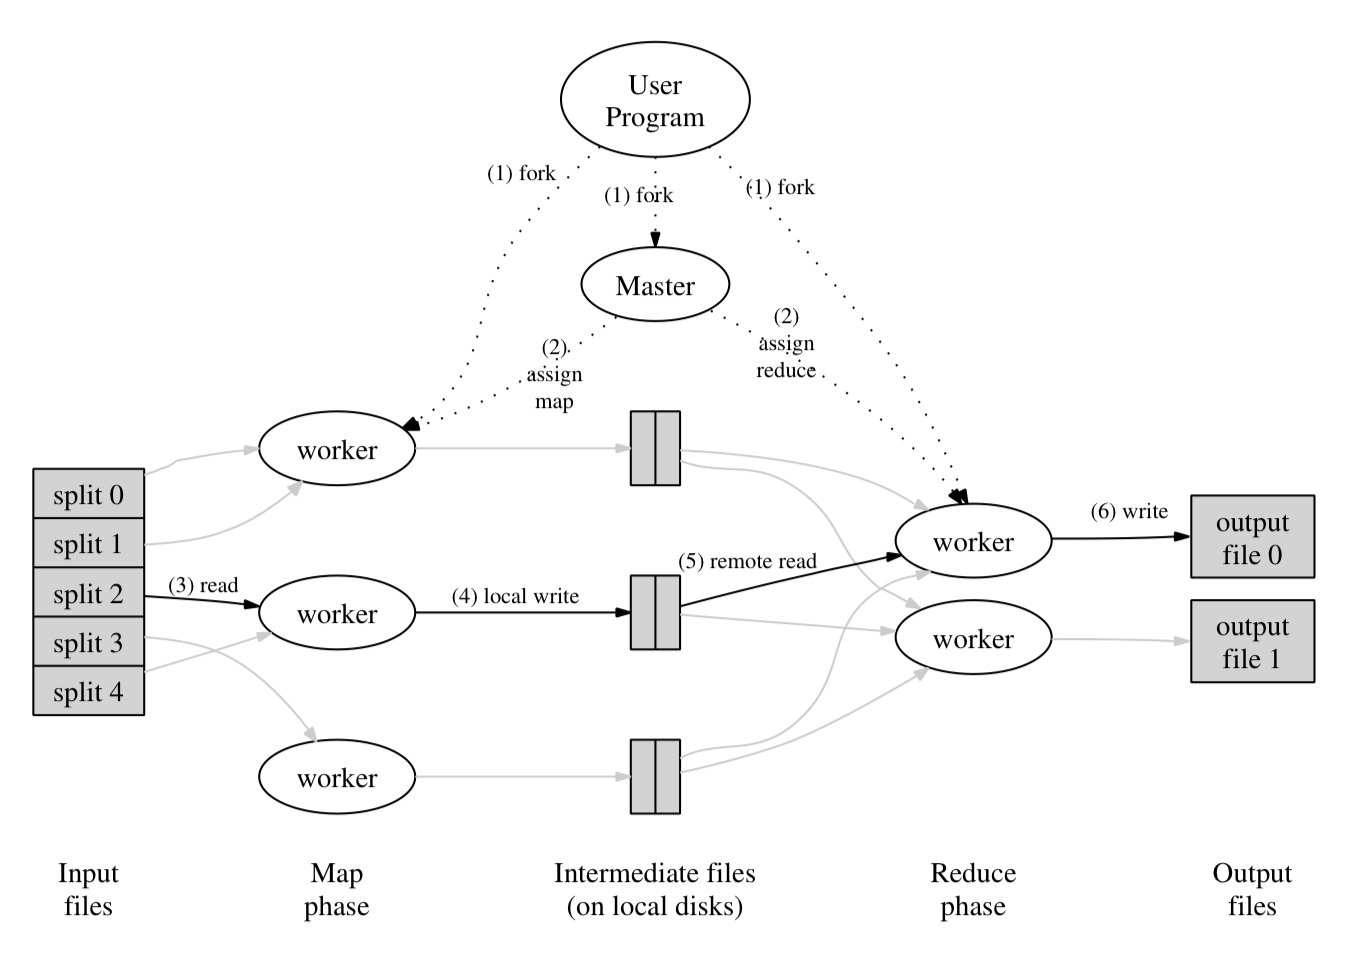
\includegraphics[width=0.85\textwidth]{map-reduce}
\caption{MapReduce 的整个流程}
\end{figure}

\begin{newnote}[MapReduce]
MapReduce 是一种编程模型。\textbf{阅读 MapReduce 论文,写阅读笔记。}  %% TODO
\end{newnote}

MapReduce 的主要问题有两个:
\begin{enumerate}
  \item 原语的语义过于低级,直接使用其来写复杂算法,开发量比较大;
  \item 依赖于磁盘进行数据传递,性能跟不上业务需求。
\end{enumerate}

为了解决 MapReduce 的两个问题,Matei 提出了一种新的数据结构 RDD%
\footnote{},
并构建了 Spark 框架。Spark 框架在 MapReduce 语义之上封装了 DAG 调度器,极大降低了算法使用的门槛。

\begin{newnote}[RDD]
RDD 弹性数据集。\textbf{阅读 Spark 论文,写阅读笔记。}  %% TODO
\end{newnote}

较长时间内 Spark 几乎可以说是大规模机器学习的代表,直至后来沐帅的参数服务器进一步开拓了大规模机器学习的领域以后,Spark 才暴露出一点点不足。如下图:

\begin{figure}[hbtp]
\centering
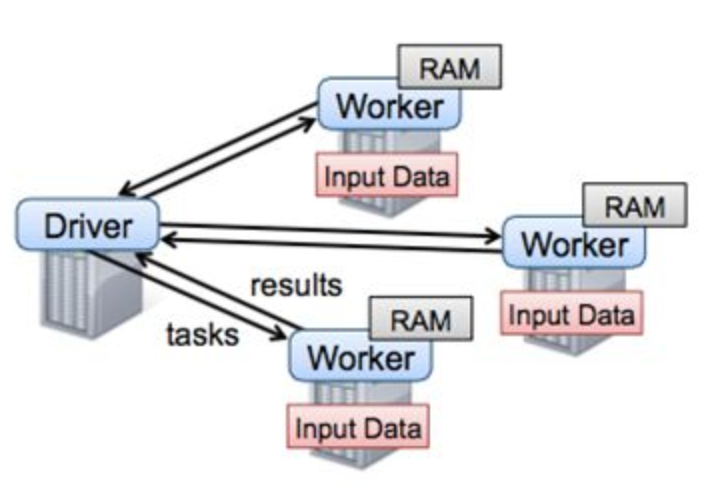
\includegraphics[width=0.65\textwidth]{spark-architecture}
\caption{Spark 的架构}
\end{figure}

从图中可以看出,Spark 框架以 Driver 为核心,任务调度和参数汇总都在 Driver,而 Driver 是单机结构,所以 Spark 的瓶颈非常明显,就在 Driver 这里。
当模型规模大到一台机器存不下的时候,Spark 就无法正常运行了。所以从今天的眼光来看,Spark 只能称为一个中等规模的机器学习框架。腾讯开源的 Angel 通过修改 Driver 的底层协议将 Spark 扩展到了一个高一层的境界。后面还会再详细介绍这部分。

\begin{newnote}[Spark]
Spark 是一个内存计算框架。
\end{newnote}

MapReduce 不仅是一个框架,还是一种思想,Google 开创性的工作为我们找到了大数据分析的一个可行方向,时至今日,仍不过时。
只是逐渐从业务层下沉到底层语义应该处于的框架下层。


\subsection{MPI技术}\label{subsec:mpi}

沐帅在知乎问题『MPI 在大规模机器学习领域的前景如何?%
\footnote{https://www.zhihu.com/question/55119470}』%
中对MPI的前景做了简要介绍:
\begin{quotation}
这个取决于场景,如果要在超算(super computer)上跑机器学习,用 MPI 是不错的选择。但在云上,不管是公有云的例如 AWS/Azure/GCP 或者私有云,MPI
没有太多必要。

MPI 定义的是接口,具体用的时候我们是用某个特定的实现,例如 openmpi 或者 mpich2。 为了简单,这里统一叫 MPI。

用  MPI 实现机器学习是没问题的,不管是对高维稀疏模型还是深度学习。MPI 的接口在一些算法的实现上很方便,另外一些地方(例如异步)绕一绕也是可以的。
例如虽然 MXNet 没有用 MPI,不过使用 MPI 来实现个 kvstore 的 backend 也是可行的。

MPI 的一大优势是支持各种网络硬件,例如 infiniband 和 Intel Omni Path,或者网络拓扑结构,例如 cray 的 dragonfly。通常 MPI 会做各种针对性的优化从而得到不错的性能。

这个优势主要体现在超算上。而对于云,通常使用常见的网络硬件(例如Ethernet)和连接结构(multi-rooted tree),MPI 做的优化通常不会有太大效果。
在云上,MPI 的一大问题是容灾。任何一个节点出问题会导致整个任务失败,会导致运营成本增加。(回答里面有提到百度有 MPI 集群。我当年是最大的用户,
一度使用超过50\% 的节点。对于这一点我是深有体会,例如凌晨 3 点起来重启任务。)

所以结论是,如果要在云上跑机器学习的话,MPI 前景不大。但如果是使用 Top500 类似的超算,MPI 是不错的选择。
\end{quotation}

和 Spark 不同,MPI 是类似 socket 的一种系统通信 API,只是支持了消息广播等功能。因为对 MPI 研究不深入,这里简单介绍下优点和缺点吧。
优点是系统级支持,性能杠杠的;缺点也比较多,一是和 MapReduce 一样因为原语过于低级,用 MPI 写算法,往往代码量比较大。另一方面是基于 MPI 的集群,
如果某个任务失败,往往需要重启整个集群,而 MPI 集群的任务成功率并不高。阿里的鲲鹏系统%
\footnote{KunPeng:Parameter Server based Distributed Learning Systems and Its Applications in
Alibaba and Ant Financial}%
给出了下图:

\begin{figure}[hbtp]
\centering
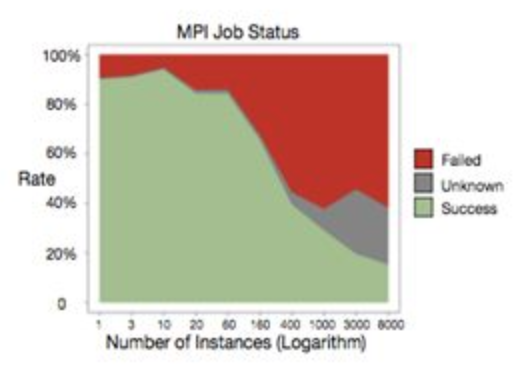
\includegraphics[width=0.85\textwidth]{mpi-task-success-rate}
\caption{MPI 集群的任务成功率}
\end{figure}

从图中可以看出,MPI 作业失败的几率接近五成。MPI 也并不是完全没有可取之处,正如沐帅所说,在超算集群上还是有场景的。对于工业届依赖于云计算、依赖于
commodity 计算机来说,则显得性价比不够高。当然如果在参数服务器的框架下,对单组 worker 再使用 MPI 未尝不是个好的尝试,鲲鹏系统正是这么设计的。

\begin{newnote}[MPI]
因为对 MPI 在之前基本就没有怎么了解过,考察一下,如果 MPI 现在使用的还比较广泛,这个可能需要整理成一个新的章节来。 %% TODO
\end{newnote}


\section{参数服务器演进}\label{subsec:ps-revolution}

\subsection{历史演进}\label{subsec:ps-history}

沐帅在 OSDI2014 的一篇文章%
\footnote{Scaling Distributed Machine Learning with the Parameter Server}% TODO 
中将参数服务器的历史划分为三个阶段,第一代参数服务器萌芽于沐帅的导师 Smola 的 paper%
\footnote{An Architecture for Parallel Topic Models}%
,如下图所示:

\begin{figure}[hbtp]
\centering
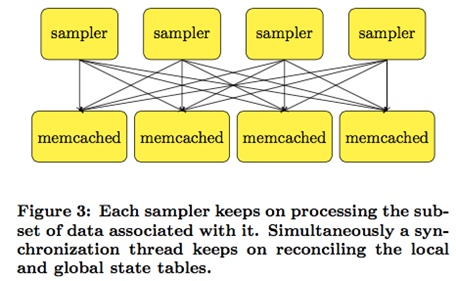
\includegraphics[width=0.85\textwidth]{topic-model}
\caption{xxxxxx待补充}
\end{figure}

这个工作中仅仅引入 memcached 来存放 key-value 数据,不同的处理进程并行对其进行处理。另一篇文章%
\footnote{Piccolo:Building fast, distributed programs with partitioned tables}%
中也有类似的想法。第二代参数服务器叫 application-specific 参数服务器,主要针对特定应用而开发,其中最典型的代表应该是 TensorFlow 的前身 DistBelief%
\footnote{Large Scale Distributed Deep Networks}。

第三代参数服务器,也即是通用参数服务器框架是由百度少帅李沐正式提出的,和前两代不同,第三代参数服务器从设计上就是作为一个通用大规模机器学习框架来定位的。
要摆脱具体应用、算法的束缚,做一个通用的大规模机器学习框架,首先就要定义好框架的功能;而所谓框架,往往就是把大量重复的、琐碎的、做了一次就不想再来第二次的脏活、累活
进行良好而优雅的封装,让使用框架的人可以只关注于自己的核心逻辑。第三代参数服务器要对哪些功能进行封装呢?沐帅总结了这几点,我照搬如下:

\begin{itemize}
  \item \textbf{高效的网络通信:}异步通信,计算与通信重叠(overlap);
  \item \textbf{灵活的一致性模型:}不同的一致性模型其实是在模型收敛速度和集群计算量之间做 tradeoff,要理解这个概念需要对模型性能的评价做些分析,
  暂且留到下节再介绍;
  \item \textbf{弹性可扩展:}新节点的加入不需要重启整个运行的框架;
  \item \textbf{容灾容错:}大规模集群协作进行计算任务的时候,出现Straggler或者机器故障是非常常见的事,因此系统设计本身就要考虑到应对;没有故障的时候,
  也可能因为对任务时效性要求的变化而随时更改集群的机器配置。这也需要框架能在不影响任务的情况下能做到机器的热插拔;
  \item \textbf{易用性:}主要针对使用框架进行算法调优的工程师而言,显然,一个难用的框架是没有生命力的。
\end{itemize}

在正式介绍第三代参数服务器的主要技术之前,先从另一个角度来看下大规模机器学习框架的演进。
 
\begin{figure}[hbtp]
\centering
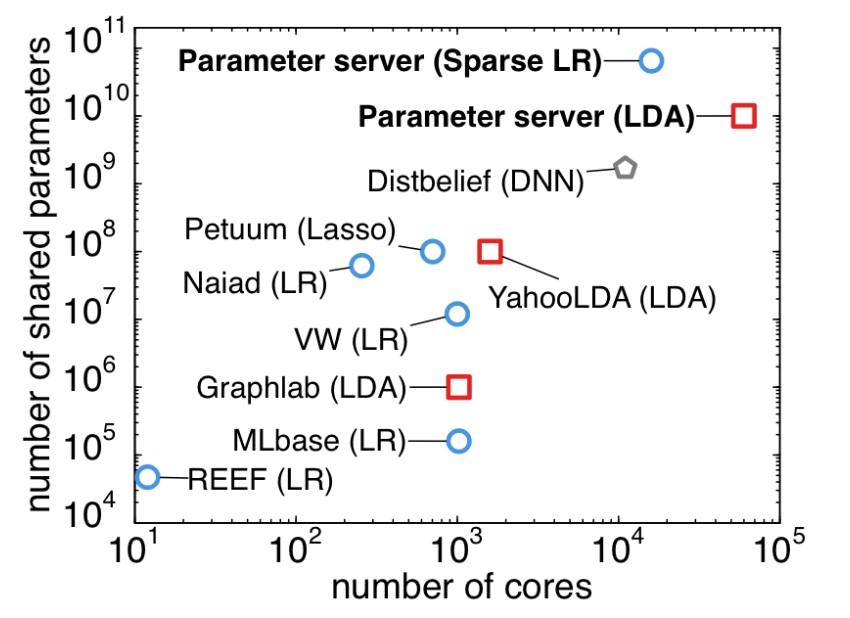
\includegraphics[width=0.65\textwidth]{ps-compare-with-others}
\caption{参数服务器与其他系统执行执行机器学习任务的比较}
\label{fig:ps-compare-with-others}
\end{figure}

这张图可以看出,在参数服务器出来之前,人们已经做了多方面的并行尝试,不过往往只是针对某个特定算法或特定领域,比如 YahooLDA 是针对 LDA 算法的。
当模型参数突破十亿以后,则可以看出参数服务器一统江湖,再无敌手。

\subsection{基础架构}\label{subsec:ps-architecture}

第三代参数服务器的基本架构

\begin{figure}[hbtp]
\centering
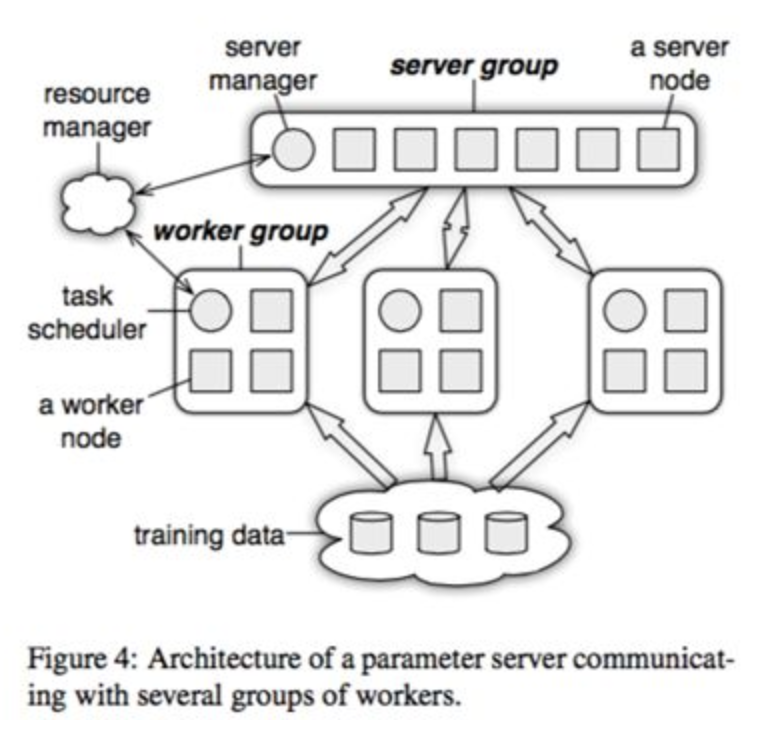
\includegraphics[width=0.85\textwidth]{ps-architecture}
\caption{xxxxxx待补充}
\end{figure}

上图的 resource manager 可以先放一放,因为实际系统中这部分往往是复用现有的资源管理系统,比如 yarn 或者 mesos;
底下的 training data 毋庸置疑的需要类似 GFS 的分布式文件系统的支持;剩下的部分就是参数服务器的核心组件了。

图中画了一个 server group 和三个 worker group;实际应用中往往也是类似,server group 用一个,而 worker group 按需配置;
server manager 是 server group 中的管理节点,一般不会有什么逻辑,只有当有 server node 加入或退出的时候,为了维持一致性哈希而做一些调整。

worker group 中的 task schedule 则是一个简单的任务协调器,一个具体任务运行的时候,task schedule 负责通知每个 worker 加载自己对应的数据,
然后去 server node 上拉取一个要更新的参数分片,用本地数据样本计算参数分片对应的变化量,然后同步给 server node;server node在收到本机负责的
参数分片对应的所有 worker 的更新后,对参数分片做一次 update。

\begin{figure}[hbtp]
\centering
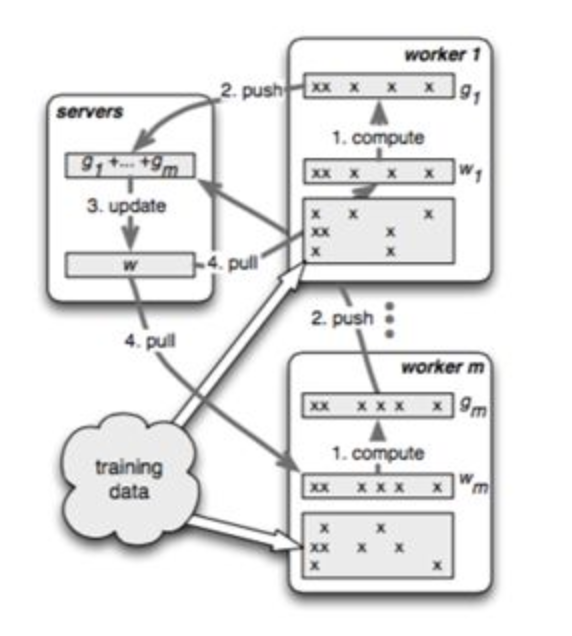
\includegraphics[width=0.65\textwidth]{ps-sub-sgd}
\caption{xxxxxx待补充}
\end{figure}

如图所示,不同的 worker 同时并行运算的时候,可能因为网络、机器配置等外界原因,导致不同的 worker 的进度是不一样的,如何控制 worker 的同步机制
是一个比较重要的课题。详见下节分解。

\textbf{ps-lite 代码详细解析}  %% TODO

\subsection{同步协议}\label{subsec:ps-synchronous}

本节假设读者已经对随机梯度优化算法比较熟悉,如果不熟悉的同学请参考吴恩达经典课程机器学习中对 SGD 的介绍,或者我之前多次推荐过的书籍
《{\color{red}最优化导论}》。

我们先看一个单机算法的运行过程,假设一个模型的参数切分成三个分片 k1,k2,k3;比如你可以假设是一个逻辑回归算法的权重向量被分成三段。我们将训练样本
集合也切分成三个分片 s1,s2,s3;在单机运行的情况下,我们假设运行的序列是(k1,s1)、(k2,s1)、(k3、s1)、(k1、s2)、(k2、s2)、(k3、s2)
$\dots$ 看明白了吗?就是假设先用 s1 中的样本一次对参数分片 k1、k2、k3 进行训练,然后换 s2;这就是典型的单机运行的情况,而我们知道这样的运行序列
最后算法会收敛。

现在我们开始并行化,假设 k1、k2、k3 分布在三个 server node 上,s1、s2、s3 分布在三个 worker node 上,这时候如果我们还要保持之前的计算顺序,
则会变成怎样?work1 计算的时候,work2 和 worker3 只能等待,同样 worker2 计算的时候,worker1 和 work3 都得等待,以此类推;可以看出这样的
并行化并没有提升性能;但是也算简单解决了超大规模模型的存储问题。

为了解决性能的问题,业界开始探索这里的一致性模型,最先出来的版本是前面提到的的ASP模式%
\footnote{An Architecture for Parallel Topic Models}% TODO 这篇文章在 TensorFlow 2016 年的文章中开始部分有提及到
,就是完全不顾 worker 之间的顺序,每个 worker 按照自己的节奏走,跑完一个迭代就 update,然后继续,这应该是大规模机器学习中的 freestyle 了,如图所示

\begin{figure}[hbtp]
\centering
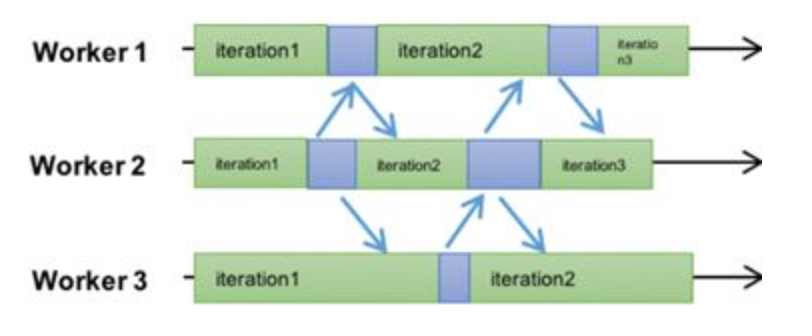
\includegraphics[width=0.85\textwidth]{asp}
\caption{ASP 模式}
\end{figure}

ASP 的优势是最大限度利用了集群的计算能力,所有的 worker 所在的机器都不用等待,但缺点也显而易见,除了少数几个模型,比如 LDA,ASP 协议可能导致模型无法收敛。
也就是 SGD 彻底跑飞了,梯度不知道飞到哪里去了。

在 ASP 之后提出了另一种相对极端的同步协议 BSP,Spark 用的就是这种方式,如图所示

\begin{figure}[hbtp]
\centering
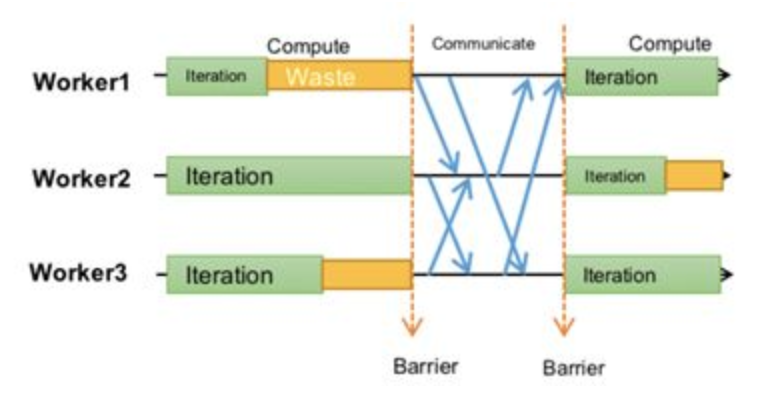
\includegraphics[width=0.85\textwidth]{bsp}
\caption{BSP 模式}
\end{figure}

每个 worker 都必须在同一个迭代运行,只有一个迭代任务所有的 worker 都完成了,才会进行一次 worker 和 server 之间的同步和分片更新。
这个算法和严格一致的算法非常类似,区别仅仅在于单机版本的 batch size 在 BSP 的时候变成了有所有 worker 的单个 batch size 求和
得到的总的 batch size 替换。毫无疑问,BSP 的模式和单机串行因为仅仅是 batch size 的区别,所以在模型收敛性上是完全一样的。同时,
因为每个 worker 在一个周期内是可以并行计算的,所以有了一定的并行能力。

以此协议为基础的 Spark 在很长时间内成为机器学习领域实际的霸主,不是没有理由的。此种协议的缺陷之处在于,整个 worker group 的性能由其中最慢的 worker 决定;这个 worker 一般称为 straggler。读过 GFS%
\footnote{The Google File System}%
文章的同学应该都知道 straggler 的存在是非常普遍的现象。

\begin{newnote}[GFS 中的 Straggler]
阅读 GFS 中的 Straggler 部分  %% TODO
\end{newnote}

能否将 ASP 和 BSP 做一下折中呢?答案当然是可以的,这就是目前我认为最好的同步协议 SSP;SSP 的思路其实很简单,既然 ASP 是允许不同 worker 之间的
迭代次数间隔任意大,而 BSP 则只允许为 0,那我是否可以取一个常数 s?如图所示

\begin{figure}[hbtp]
\centering
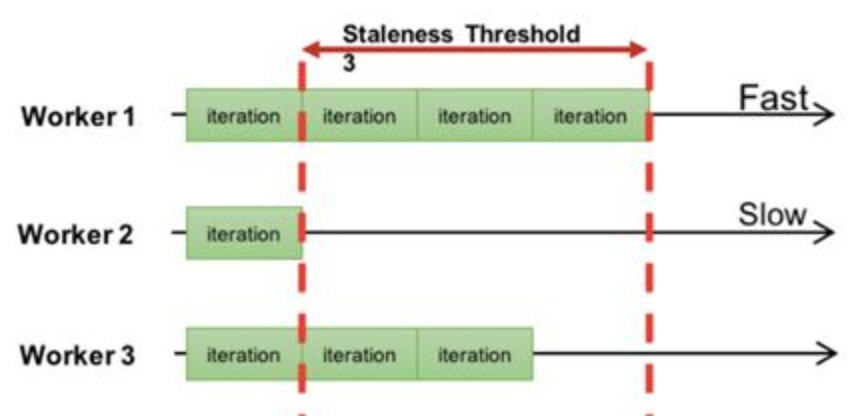
\includegraphics[width=0.85\textwidth]{ssp}
\caption{SSP 模式}
\end{figure}

不同的 worker 之间允许有迭代的间隔,但这个间隔数不允许超出一个指定的数值 s,图中 s=3.

SSP 协议的详细介绍参见%
\footnote{More Effective Distributed ML via a Stale Synchronous Parallel Parameter Server}%  TODO 这篇文章真是很有开创性啊!
,CMU 的大拿 Eric Xing 在其中详细介绍了 SSP 的定义,以及其收敛性的保证。理论推导证明常数 s 不等于无穷大的情况下,算法一定可以在若干次迭代以后进入收敛状态。
其实在 Eric 提出理论证明之前,工业界已经这么尝试过了:)

\begin{newnote}[从另一个角度看数据并行]
在随机梯度下降中,数据并行使用参数服务器(Parameter Server)来做同步,同步的策略就是我们上面提到的 ASP、BSP 以及 SSP。在 GeePS
中,提到同步策略对更新效率的影响,BSP 最好,SSP 次优,ASP 最差;但 BSP 每轮都需要同步,训练一批数据时间会最长,SSP 次优,ASP 最快。
所以这就是一个 tradeoff 的问题了:如何选择同步策略?

GeePS: Scalable deep learning on distributed GPUs with a GPU-specialized parameter server  %% TODO

整理自:https://www.zhihu.com/question/31999064/answer/106715799
\end{newnote}

\begin{figure}[hbtp]
\centering
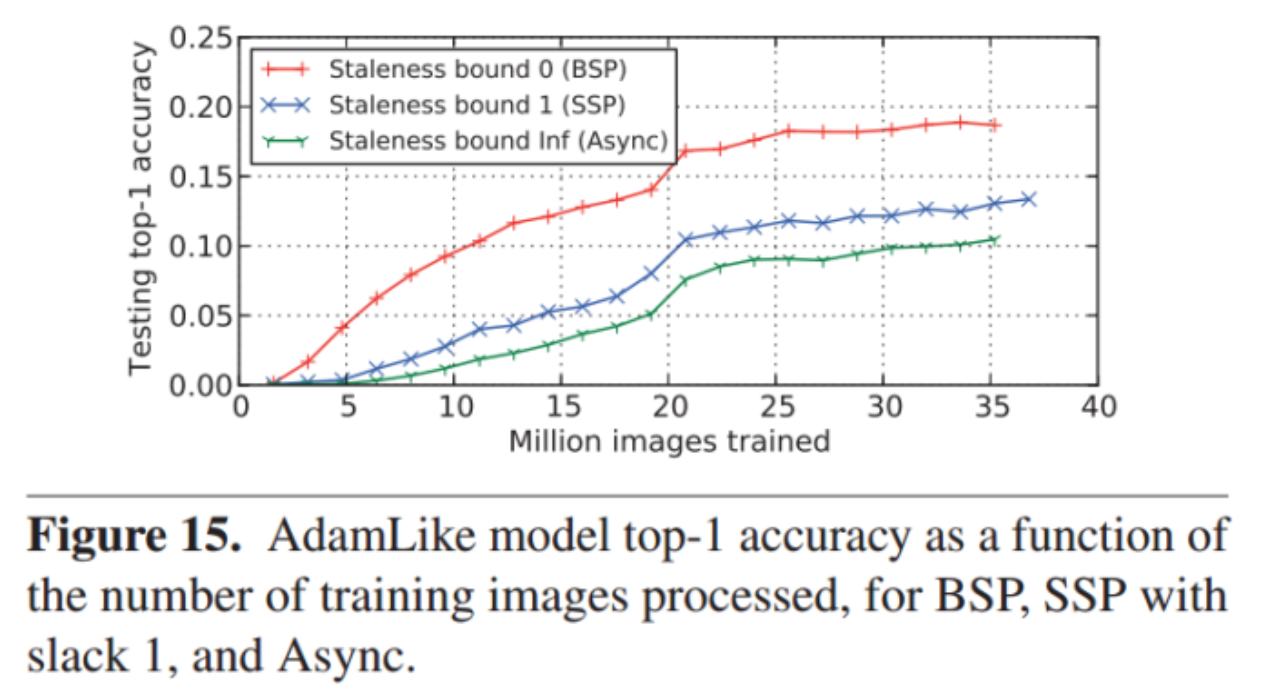
\includegraphics[width=0.85\textwidth]{asp-bsp-ssp}
\caption{ASP、BSP 以及 SSP 各同步策略对更新效率的影响}
\end{figure}

顺便提一句,考察分布式算法的性能,一般会分为 statistical performance 和 hard performance 来看。前者指不同的同步协议导致算法收敛需要的迭代次数的多少,
后者是单次迭代所对应的耗时。两者的关系和 precision/recall 关系类似,就不赘述了。有了 SSP,BSP 就可以通过指定 s=0 而得到。而 ASP 同样可以通过指定
s=$\infty$ 来达到。

\subsection{核心技术}\label{subsec:ps-cores}

除了参数服务器的架构、同步协议之外,本节再对其他技术做一个简要的介绍,详细的了解请直接阅读沐帅的博士论文和相关发表的论文% TODO
\footnote{http://www.cs.cmu.edu/\~muli/}。

热备、冷备技术:为了防止 server node 挂掉,导致任务中断,可以采用两个技术,一个是对参数分片进行热备,每个分片存储在三个不同的 server node 中,以 master-slave 的形式存活。如果 master 挂掉,可以快速从 slave 获取并重启相关 task。除了热备,还可以定时写入 checkpoint 文件到分布式文件系统来对参数分片及其状态进行备份。
进一步保证其安全性。

server node 管理:可以使用一致性哈希技术来解决 server node 的加入和退出问题,如图所示 
%% TODO 一致性哈希的方法,可以整理到第三章中,分布式系统中需要考虑的几个要素

\begin{figure}[hbtp]
\centering
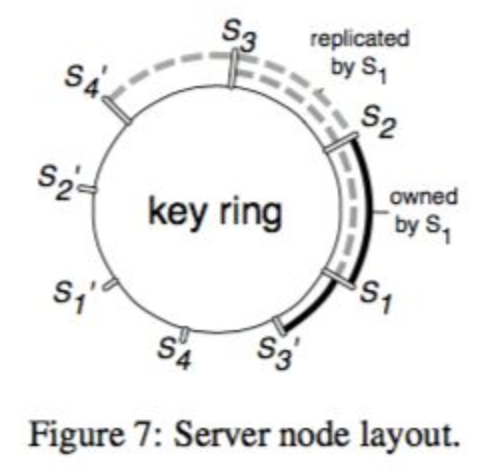
\includegraphics[width=0.65\textwidth]{server-node-layout}
\caption{Server node layout}
\end{figure}

当有 server node 加入或退出的时候,server manager 负责对参数进行重新分片或者合并。注意在对参数进行分片管理的情况下,一个分片只需要一把锁,
这大大提升了系统的性能,也是参数服务器可以实用的一个关键点。


\noindent\rule[0.25\baselineskip]{\textwidth}{1pt}

\section{大规模机器学习的四重境界}\label{sec:three-of-four}

到这里可以回到我们的标题了,大规模机器学习的四重境界到底是什么呢?这四重境界的划分是作者个人阅读总结的一种想法,并不是业界标准,仅供大家参考。

\subsection{境界 1}\label{subsec:first}

\noindent\textbf{参数可单机存储和更新}

此种境界较为简单,但仍可以使用参数服务器,通过数据并行来加速模型的训练。

\subsection{境界 2}\label{subsec:second}

\noindent\textbf{参数不可单机存储,可以单机更新}

此种情况对应的是一些简单模型,比如 sparse logistic regression;当 feature 的数量突破百亿的时候,LR 的权重参数
不太可能在一台机器上完全存下,此时必须使用参数服务器架构对模型参数进行分片。但是注意一点,SGD 的更新公式

\begin{equation*}
w^{\rq} = w - \alpha
\end{equation*}

其中可以分开到单个维度进行计算,但是单个维度的 $w_i = f(x)x_i$。

这里的 $f(w)$ 表示是全部参数 w 的一个函数,具体推导比较简单,这里篇幅所限就不赘述了。只是想说明 worker 在计算梯度的时候可能需要使用到
上一轮迭代的所有参数。而我们之所以对参数进行分片就是因为我们无法将所有参数存放到一台机器,现在单个 worker 有需要使用所有的参数
才能计算某个参数分片的梯度,这不是矛盾吗?可能吗?

答案是可能的,因为单个样本的 feature 具有很高的稀疏性(sparseness)。例如一个百亿 feature 的模型,单个训练样本往往只在其中很小
一部分 feature 上有取值,其他都为 0(假设 feature 取值都已经离散化了)。因此计算 $f(w)$ 的时候可以只拉取不为 0 的 feature 对应的
那部分 w 即可。有文章统计一般这个级别的系统,稀疏性往往在0.1\%(or 0.01\%,记得不是很准,大致这样)以下。这样的稀疏性,
可以让单机没有任何阻碍的计算 $f(w)$。

目前腾讯开源的 Angel 和 AILab 正在做的系统都处于这个境界。而原生 Spark 还没有达到这个境界,只能在中小规模的圈子里厮混。

\subsection{境界 3}\label{subsec:third}

\noindent\textbf{参数不可单机存储,不可单机更新,但无需模型并行}

境界 3 顺延境界 2 而来,当百亿级 feature 且 feature 比较稠密的时候,就需要计算框架进入到这层境界了,此时单个 worker 的能力有限,
无法完整加载一个样本,也无法完整计算 $f(w)$。怎么办呢?其实很简单,学过线性代数的都知道,矩阵可以分块。向量是最简单的矩阵,自然可以切成
一段一段的来计算。只是调度器需要支持算符分段而已了。

\subsection{境界 4}\label{subsec:fourth}

\noindent\textbf{参数不可单机存储,不可单机更新,需要模型并行}

进入到这个层次的计算框架,可以算是世界一流了。可以处理超大规模的神经网络。这也是最典型的应用场景。此时不仅模型的参数不能单机存储,
而且同一个迭代内,模型参数之间还有强的依赖关系,可以参见姐夫对 Distbelief 的介绍里的模型切分。

此时首先需要增加一个 coordinator 组件来进行模型并行的 concurrent 控制。同时参数服务器框架需要支持 namespace 切分,coordinator
将依赖关系通过 namespace 来进行表示。

一般参数间的依赖关系因模型而已,所以较难抽象出通用的 coordinator 来,而必须以某种形式通过脚本 parser 来生产整个计算任务的 DAG 图,然后通过 DAG 调度器来完成。对这个问题的介绍可以参考Erix Xing的分享\footnote{https://www.jianshu.com/p/00736aa21dc8}。

\subsection{TensorFlow}\label{subsec:tensorflow}

目前业界比较知名的深度学习框架有 Caffe、MXNet、Torch、Keras、Theano等,但目前最炙手可热的应该是 Google 发布的 TensorFlow。这里单独拿出来稍微分解下。

前面不少图片引自此文%
\footnote{TensorFlow:Large-Scale Machine Learning on Heterogeneous Distributed Systems}%
,从 TF 的论文来看,TF 框架本身是支持模型并行和数据并行的,内置了一个参数服务器模块,但从开源版本所曝光的 API 来看,TF 无法用来 10B 级别 feature
的稀疏 LR 模型。原因是已经曝光的 API 只支持在神经网络的不同层和层间进行参数切分,而超大规模 LR 可以看做一个神经单元,TF 不支持单个神经单元参数
切分到多个参数服务器 node 上。

当然,以 Google 的实力,绝对是可以做到第四重境界的,之所以没有曝光,可能是基于其他商业目的的考量,比如使用他们的云计算服务。

综上,个人认为如果能做到第四重境界,目前可以说的上是世界一流的大规模机器学习框架。仅从沐帅的 ppt 里看他曾经达到过,Google 内部应该也是没有问题的。
第三重境界应该是国内一流,第二充应该是国内前列吧。


\section{其他}\label{sec:other}

\subsection{资源管理}\label{subsec:resource-management}

本文没有涉及到的部分是资源管理,大规模机器学习框架部署的集群往往资源消耗也比较大,需要专门的资源管理工具来维护。这方面 yarn 和 mesos 都是佼佼者,
细节这里也就不介绍了

\subsection{设备}\label{subsec:devices}

除了资源管理工具,本身部署大规模机器学习集群本身对硬件也还是有些要求的,虽然理论上来说,所有 commodity 机器都可以用来搭建这类集群,但是考虑到性能,
我们建议尽量用高内存的机器+万兆及以上的网卡。没有超快速的网卡,玩参数传递和样本加载估计会比较苦逼。


\section{结语}\label{sec:another}

从后台转算法以来,长期沉浸于算法推理的论文无法自拔,对自己之前的后台工程能力渐渐轻视起来,觉得工程对算法的帮助不大。直到最近一个契机,
需要做一个这方面的调研,才豁然发现,之前的工程经验对我理解大规模机器学习框架非常有用,果然如李宗盛所说,人生每一步路,都不是白走的。

在一个月左右的调研中,脑子每天都充斥这各种疑问和困惑,曾经半夜4点醒来,思考同步机制而再也睡不着,干脆起来躲卫生间看书,而那天我一点多才睡。
当脑子里有放不下的问题的时候,整个人会处于一种非常亢奋的状态,除非彻底想清楚这个问题,否则失眠是必然的,上一次这种状态已经是很多年前了。
好在最后我总算理清了这方面的所有关键细节。以此,记之。Carbonzhang 于 2017 年 8 月 26 日凌晨!


\section*{致谢}

感谢 wills、janwang、joey、roberty、suzi 等同学一起讨论,特别感谢 burness 在 TF 方面的深厚造诣和调研。因为本人水平所限,错漏难免,
另外还有相当多的细节因为篇幅限制并未一一展开,仅仅是从较高抽象层面上简述了下大规模机器学习框架的关键思路,其他如分片向量锁、通信协议、时钟逻辑、
DAG 调度器、资源调度模块等均为展开来讲,希望以后有机会能补上。

\endinput
